\chapter{The nuclear model with explicit mesons}\label{Decsofmodel}

We consider a nuclear model where the nucleus is held together by emitting and absorbing mesons, and the mesons are treated explicitly \cite[]{Mesons}. We are considering the regime of low-energy nuclear physics, and this model is different from conventional interaction models in several ways. Firstly, the nucleons interact by emitting and absorbing mesons and not via a phenomenological potential. Conceptually this is similar to the one-boson-exchange model. Secondly, the number of parameters is greatly reduced. Regardless of the meson type, the number of parameters is two; the range and the strength of the meson-nucleon coupling are denoted $b$ and $S$, respectively. In the case of the pion, the central force, tensor force and the three-body force are all concealed within these two parameters. This model should be able to reproduce phenomena within the realm of low-energy nuclear physics, such as the deuteron, nucleon-nucleon scattering, pion-nucleon scattering and pion photoproduction. The low energy regime also enables the use of the Schrödinger equation to describe the equations of motion. The model must be constructed in a way such that usual quantum numbers are conserved; this means conservation of isospin, angular momentum and parity. 

\section{Nuclear interacting model with explicit pions }\label{sec:model}

In the following, we focus on the nuclear model with explicit pions. The pion is the lightest of the strongly interacting particles with a mass of about $15\%$ of the nucleon mass. This yields a large Compton wavelength of $1.4$ fm, which means the most extended contribution to nucleon-nucleon interactions. Furthermore, the pion is a significant component of the nuclear wave function where the pion dominates meson exchange corrections to different nuclear properties. In general, the bare nucleon is surrounded by several virtual pions. 
They are virtual in the same sense that the positron-electron pair are virtual in pair creation from a photon. It is important to stress that these are virtual since they can have properties possible for true particles. The multi-component wave function of the nucleon can be written as
\begin{marginfigure}
	\centering
	

\tikzset{every picture/.style={line width=0.75pt}} %set default line width to 0.75pt        

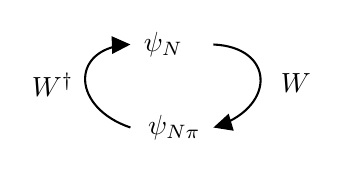
\begin{tikzpicture}[x=0.75pt,y=0.75pt,yscale=-1,xscale=1]
	%uncomment if require: \path (0,300); %set diagram left start at 0, and has height of 300
	
	%Curve Lines [id:da45911359937309637] 
	\draw    (280,60) .. controls (309.18,61.28) and (310.43,89.17) .. (282.66,99.13) ;
	\draw [shift={(280,100)}, rotate = 343.41] [fill={rgb, 255:red, 0; green, 0; blue, 0 }  ][line width=0.08]  [draw opacity=0] (8.93,-4.29) -- (0,0) -- (8.93,4.29) -- cycle    ;
	%Curve Lines [id:da6231994153364976] 
	\draw    (240,100) .. controls (211.9,90.47) and (210.92,62.94) .. (237.05,60.2) ;
	\draw [shift={(240,60)}, rotate = 178.19] [fill={rgb, 255:red, 0; green, 0; blue, 0 }  ][line width=0.08]  [draw opacity=0] (8.93,-4.29) -- (0,0) -- (8.93,4.29) -- cycle    ;
	
	% Text Node
	\draw (245,52.4) node [anchor=north west][inner sep=0.75pt]    {$\psi _{N}$};
	% Text Node
	\draw (247,92.4) node [anchor=north west][inner sep=0.75pt]    {$\psi _{N\pi }$};
	% Text Node
	\draw (191,72.4) node [anchor=north west][inner sep=0.75pt]    {$W^{\dagger }$};
	% Text Node
	\draw (311,72.4) node [anchor=north west][inner sep=0.75pt]    {$W$};
	
	
\end{tikzpicture}
	\caption{Illustration of the pion-nucleon operator, $W$}
	\label{fig:superposition}
\end{marginfigure}

\begin{equation} \label{superposition}
	\Psi_N = \mqty[\psi_{N} \\
	\psi_{N\pi} \\
	\psi_{N\pi\pi}\\
	\vdots],
\end{equation}
where $\psi_{N}$ is the bare nucleon, and the other wave functions are dressed by an arbitrary number of pions indicated by the subscripts. Assuming the nuclear interaction conserved isospin, angular momentum and parity, we can construct the following operator for the pion-nucleon operator
\begin{align} \label{W}
	W & \equiv (\vec{\tau\cdot\vec{\pi}})(\vec{\sigma}\cdot\vec{r})f(r) \\
	W^\dagger & \equiv  \int_V \text{d}^3 r \, (\vec{\tau\cdot\vec{\pi}})^\dagger (\vec{\sigma}\cdot\vec{r})^\dagger f(r) \label{Wdagger},
\end{align}
where $\vec{\tau}$ is the isovector of Pauli matrices acting on the nucleon in isospin space and $\vec{\sigma}$ is the same but for spin space and $\vec{r}$ is the relative coordinate distance between the nucleon and the pion. These operators ensure the conservation of isospin, angular momentum and parity. The isovector of pions is denoted $\vec{\pi}$ and can be combined with $\vec{\tau}$ and be represented as a traceless 2-by-2 hermitian matrix given by
\begin{equation} \label{isocoeff}
	\vec{\tau}\cdot \vec{\pi} = \tau_0  \pi_0+ \sqrt{2} \tau_{-}\pi^ +\sqrt{2}\tau_{+} \pi^{-} = \mqty[\pi^0 & \sqrt{2}\pi^- \\
	\sqrt{2}\pi^+ & -\pi^0],
\end{equation}
where the isospin coefficients will be important later when we discuss different photoproduction processes. Similarly, by expanding the matrices in spin space and using the spherical tensor operator, we get the following matrix in terms of the spherical harmonics
\begin{equation}\label{spinmatrix}
	\vec{\sigma}\cdot \vec{r} = \sqrt{\frac{4\pi}{3}} r \mqty[Y_{1}^0 & \sqrt{2}Y_1^{-1} \\ \sqrt{2}Y_1^1 & Y_1^0],
\end{equation}
where similar to in isospin space, the off-diagonals include a factor $\sqrt{2}$.  
\begin{marginfigure}
	\centering
	

\tikzset{every picture/.style={line width=0.75pt}} %set default line width to 0.75pt        

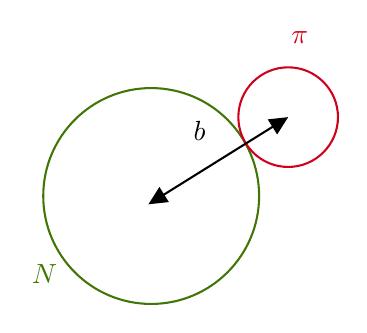
\begin{tikzpicture}[x=0.75pt,y=0.75pt,yscale=-1,xscale=1]
%uncomment if require: \path (0,300); %set diagram left start at 0, and has height of 300

%Shape: Circle [id:dp5217046923283729] 
\draw  [color={rgb, 255:red, 65; green, 117; blue, 5 }  ,draw opacity=1 ] (177,163) .. controls (177,134.28) and (200.28,111) .. (229,111) .. controls (257.72,111) and (281,134.28) .. (281,163) .. controls (281,191.72) and (257.72,215) .. (229,215) .. controls (200.28,215) and (177,191.72) .. (177,163) -- cycle ;
%Shape: Circle [id:dp22288734190325] 
\draw  [color={rgb, 255:red, 208; green, 2; blue, 27 }  ,draw opacity=1 ] (271,125) .. controls (271,111.75) and (281.75,101) .. (295,101) .. controls (308.25,101) and (319,111.75) .. (319,125) .. controls (319,138.25) and (308.25,149) .. (295,149) .. controls (281.75,149) and (271,138.25) .. (271,125) -- cycle ;
%Straight Lines [id:da9107173582949104] 
\draw    (230.21,165.41) -- (292.45,126.59) ;
\draw [shift={(295,125)}, rotate = 148.05] [fill={rgb, 255:red, 0; green, 0; blue, 0 }  ][line width=0.08]  [draw opacity=0] (8.93,-4.29) -- (0,0) -- (8.93,4.29) -- cycle    ;
\draw [shift={(227.67,167)}, rotate = 328.05] [fill={rgb, 255:red, 0; green, 0; blue, 0 }  ][line width=0.08]  [draw opacity=0] (8.93,-4.29) -- (0,0) -- (8.93,4.29) -- cycle    ;

% Text Node
\draw (170,194.4) node [anchor=north west][inner sep=0.75pt]  [color={rgb, 255:red, 65; green, 117; blue, 5 }  ,opacity=1 ]  {$N$};
% Text Node
\draw (295,82.4) node [anchor=north west][inner sep=0.75pt]  [color={rgb, 255:red, 208; green, 2; blue, 27 }  ,opacity=1 ]  {$\pi$};
% Text Node
\draw (248,125.4) node [anchor=north west][inner sep=0.75pt]  [color={rgb, 255:red, 0; green, 0; blue, 0 }  ,opacity=1 ]  {$b$};


\end{tikzpicture}
	\caption{Schematic figure of the system to describe the form factor, \eqref{formfactoreq}. The pion is assumed to sit on the surface.}
	\label{formfactor}
\end{marginfigure}
There is also a phenomenological, short-range form factor $f(r)$ given by
\begin{equation}\label{formfactoreq}
	f(r) = \frac{S}{b} \text{e}^{-r^2/b^2},
\end{equation}
where $S$ and $b$ are the pion-nucleon coupling strength and range, respectively--these are illustrated in figure \ref{formfactor}. The action of annihilating a pion must include the integral over coordinate space to remove the coordinate. We now have everything we need to construct a general Hamiltonian for the multi-component wave function of the nucleon in \eqref{superposition}
\begin{equation} \label{multihamiltonian}
	H = \mqty[K_N & W^\dagger & 0 &\ldots \\
	W & K_N+K_\pi+m_\pi c^2+V_C & W^\dagger & \ldots \\
	0 & W & K_N+K_{\pi(1)}+K_{\pi(2)}+2m_\pi c^2 +V_C & \ldots \\
	\vdots & \vdots & \vdots &\ddots ],
\end{equation}
where the kinetic operators are given by
\begin{align} \label{multiN}
	K_N &= \frac{-\hbar^2}{2 m_N c^2} \frac{\partial}{\partial \vec{R}^2} \\
	K_\pi &= \frac{-\hbar^2}{2 m_\pi c^2} \frac{\partial}{\partial \vec{r}^2} \label{kinpi}.
\end{align} 
Note the different derivatives--here $\vec{R}$ is the centre-of-mass coordinate, and $\vec{r}$ is the relative coordinate. The subscripts on the kinetic operators in \eqref{multihamiltonian} represent the order in which the pions are created. Should there be charged particles involved, one must include a Coulomb interaction denoted by $V_C$. From \eqref{superposition} and \eqref{multihamiltonian} we can construct the general Schrödinger equation
\begin{equation} \label{MultiSE}
	H \Psi_N = E \Psi_N,
\end{equation}
where the ground state is the bare nucleon surrounded by virtual pions. The ground state energy in the rest frame of the nucleon gives the mass of the physical nucleon. Within the framework of this model, one can generate a physical pion by supplying enough energy such that the pion is no longer virtual. The pion is trapped behind a potential barrier of height $m_\pi c^2 = 140$ MeV and cannot leave unless this or more energy is supplied to the system.  
\section{Dressing of the nucleon in the one pion approximation}\label{dressnuc}
\begin{marginfigure}
	\centering
	

\tikzset{every picture/.style={line width=0.75pt}} %set default line width to 0.75pt        

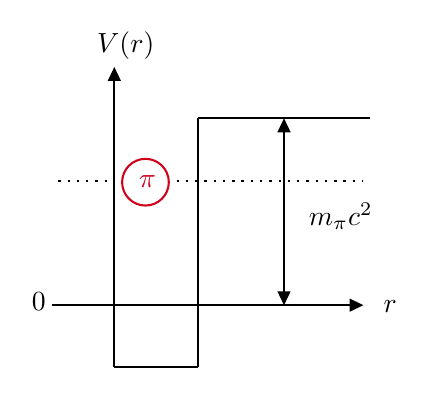
\begin{tikzpicture}[x=0.75pt,y=0.75pt,yscale=-0.75,xscale=0.75]
	%uncomment if require: \path (0,462); %set diagram left start at 0, and has height of 462
	
	%Straight Lines [id:da04487003009359902] 
	\draw    (276,240) -- (276,90) ;
	\draw [shift={(276,87)}, rotate = 90] [fill={rgb, 255:red, 0; green, 0; blue, 0 }  ][line width=0.08]  [draw opacity=0] (8.93,-4.29) -- (0,0) -- (8.93,4.29) -- cycle    ;
	%Straight Lines [id:da11984458862135328] 
	\draw    (236,240) -- (433,240) ;
	\draw [shift={(436,240)}, rotate = 180] [fill={rgb, 255:red, 0; green, 0; blue, 0 }  ][line width=0.08]  [draw opacity=0] (8.93,-4.29) -- (0,0) -- (8.93,4.29) -- cycle    ;
	%Straight Lines [id:da39644848633047847] 
	\draw    (330,280) -- (330,120) ;
	%Straight Lines [id:da23479083436400994] 
	\draw    (330,280) -- (297,280) -- (276,280) ;
	%Straight Lines [id:da22091112894519627] 
	\draw    (276,240) -- (276,280) ;
	%Straight Lines [id:da47586844464292766] 
	\draw  [dash pattern={on 0.84pt off 2.51pt}]  (240,160) -- (276,160) ;
	%Straight Lines [id:da07090607985351194] 
	\draw  [dash pattern={on 0.84pt off 2.51pt}]  (316,160) -- (436,160) ;
	%Flowchart: Connector [id:dp0772408562939938] 
	\draw  [color={rgb, 255:red, 208; green, 2; blue, 27 }  ,draw opacity=1 ] (281,161) .. controls (281,152.72) and (287.72,146) .. (296,146) .. controls (304.28,146) and (311,152.72) .. (311,161) .. controls (311,169.28) and (304.28,176) .. (296,176) .. controls (287.72,176) and (281,169.28) .. (281,161) -- cycle ;
	%Straight Lines [id:da8208549108465544] 
	\draw    (330,120) -- (440,120) ;
	%Straight Lines [id:da059140841724983684] 
	\draw    (385,237) -- (385,123) ;
	\draw [shift={(385,120)}, rotate = 90] [fill={rgb, 255:red, 0; green, 0; blue, 0 }  ][line width=0.08]  [draw opacity=0] (8.93,-4.29) -- (0,0) -- (8.93,4.29) -- cycle    ;
	\draw [shift={(385,240)}, rotate = 270] [fill={rgb, 255:red, 0; green, 0; blue, 0 }  ][line width=0.08]  [draw opacity=0] (8.93,-4.29) -- (0,0) -- (8.93,4.29) -- cycle    ;
	
	% Text Node
	\draw (263,62.4) node [anchor=north west][inner sep=0.75pt]    {$V(r)$};
	% Text Node
	\draw (447,235) node [anchor=north west][inner sep=0.75pt]    {$r$};
	% Text Node
	\draw (290,155) node [anchor=north west][inner sep=0.75pt]  [color={rgb, 255:red, 208; green, 2; blue, 27 }  ,opacity=1 ]  {$\pi $};
	% Text Node
	\draw (221,230) node [anchor=north west][inner sep=0.75pt]    {$0$};
	% Text Node
	\draw (399,172.4) node [anchor=north west][inner sep=0.75pt]    {$m_{\pi } c^{2}$};
	
	
\end{tikzpicture}
	\caption{Illustration of the virtual pion}
	\label{fig:Underbarrier}
\end{marginfigure}
We now consider the scenario where a photon interacts with the nucleon-pion systems and generates a physical pion. This means the energy is higher than the potential barrier also when taking recoil effects into account. This also hints at how a pion photoproduction process would emerge naturally as a disintegration process in this nuclear model. To generate more pions, the photon energy would have to be increased by the same amount. This also means one could assume the first pion is responsible for the largest contribution to the nucleon dressing. This will be referred to as the one-pion approximation. As a proof-of-concept, we constrain ourselves to the one pion approximation and adding more pions should in principle be a straight forward extension of the following calculations.

Returning to \eqref{superposition} and enforcing the one-pion approximation yields
\begin{equation} \label{2wavefunc}
	\Psi = \mqty[\psi_{N}(\vec{R})\\
	\psi_{N\pi}(\vec{r})].
\end{equation}
The Hamiltonian which acts on the two-component wave function in \eqref{2wavefunc} is given by\footnote{Strictly speaking one should use a three-component wave function to account for the mass difference between $\pi^0$ and $\pi^\pm$. This is done in appendix \ref{ThreeComponentWavefunction}.}
\begin{equation}\label{HamilTwo}
	H  =  \mqty[K_N & W^\dagger \\ W & K_N+K_\pi+m_\pi c^2],
\end{equation}
So far we have kept the model as simple as possible by expressing the equations in terms of the nucleon. From now on we treat the nucleon of two states of the same strongly interacting object with an intrinsic degree of freedom which defines the proton and neutron. We choose the proton and neutron as 
\begin{equation} \label{isospinvec}
	\ket{p} = \mqty[1 \\ 0 ] \quad \ket{n} = \mqty[0 \\ 1].
\end{equation} 
Furthermore, we denote the spin state of the nucleon by an arrow
\begin{equation} \label{spinvec}
	\uparrow = \mqty[1 \\ 0 ] \quad  \downarrow= \mqty[0 \\ 1].
\end{equation}
The wave function must also be normalized to one nucleon per unit volume. This is as far as we get in general terms for the dressing of the nucleon in the one-pion approximation.
\section{Dressing of the proton} \label{sec:DressingofProton}
We now focus our attention on the dressing of the proton in the spin-up state. The calculations are almost identical remembering the definitions from section \ref{dressnuc}. The wave function of the bare proton can thus be written as
\begin{equation} \label{bareproton}
	\psi_p = \frac{p\uparrow}{\sqrt{V}}
\end{equation}
The Hamiltonian \eqref{HamilTwo} suggest the following expression for the wave function of the pion-nucleon system
\begin{equation} \label{pionnuc}
	\psi_{N\pi} = (\vec{\tau}\cdot\vec{\pi})(\vec{\sigma}\cdot\vec{r})\frac{p \uparrow}{\sqrt{V}}\phi(r),
\end{equation}
where $\phi(r)$ is the radial function which will play an integral part in the rest of this section.
From \eqref{W} we can construct the Schrödinger equation of the system
\begin{equation}\label{SE}
	\mqty[K_{p} & W^\dagger \\ W & K_{N}+K_{\pi}+m_\pi c^2]\mqty[\psi_p \\ \psi_{N\pi}] = E \mqty[\psi_p \\ \psi_{N\pi}].
\end{equation}
Note that the kinetic operator in the second row still contains $K_N$ to emphasise that this acts on the general nucleon-pion wave function, $\psi_{N\pi}$. Expanding \eqref{SE} yields two equations
\begin{align}
	K_{p}\psi_p + W^\dagger \psi_{N\pi} & = E\psi_p \label{SE1} \\
	W\psi_p + (K_{N}+K_{\pi}+m_\pi c^2)\psi_{N\pi} & = E\psi_{N\pi} \label{SE2}.
\end{align}
In the rest frame of the proton the center-of-mass dependency vanishes and inserting the operator \eqref{W} yields
\begin{equation}
	\int_V \text{d}^3r \, (\vec{\tau\cdot\vec{\pi}})^\dagger(\vec{\sigma}\cdot\vec{r})^\dagger f(r)\phi(r)(\vec{\tau\cdot\vec{\pi}})(\vec{\sigma}\cdot\vec{r})p\frac{1}{\sqrt{V}} = E p\frac{1}{\sqrt{V}},
\end{equation}
where the integration comes from equation \eqref{Wdagger}. This can be further simplified using relations for the matrix vectors\footnote{$(\vec{\tau}\cdot \vec{\pi})^\dagger(\vec{\tau}\cdot \vec{\pi}) = 3$ \\ and
	$(\vec{\sigma}\cdot \vec{r})^\dagger(\vec{\sigma}\cdot \vec{r}) = r^2$}
\begin{equation} \label{SE11}
	12\pi \int_0^\infty  \text{d}r \, f(r) \phi(r) r^4  = E.
\end{equation}
Similarly for \eqref{SE2} where the term $K_{N}\psi_{N\pi}$ vanishes,
\begin{equation}\begin{split}\label{SE22}
		(\vec{\tau\cdot\vec{\pi}})(\vec{\sigma}\cdot\vec{r})f(r) p \frac{1}{\sqrt{V}}-\frac{\hbar^2}{2\mu_{N\pi}} \nabla^2_{\vec{r}}(\vec{\tau\cdot\vec{\pi}})(\vec{\sigma}\cdot\vec{r}) p \frac{1}{\sqrt{V}}\phi(r) \\ \quad= (E-m_\pi c^2) (\vec{\tau\cdot\vec{\pi}})(\vec{\sigma}\cdot\vec{r}) \phi(r)p\frac{1}{\sqrt{V}},
	\end{split}
\end{equation}
using \eqref{kinpi} and where $\mu_{N\pi}$ is the reduced mass of the nucleon-pion system. This equation can be further simplified by using a vector operator relation which yields\footnote{$\nabla^2(\vec{r}\phi(r))=\vec{r}\big(\frac{\text{d}^2\phi(r)}{\text{d}r^2}+\frac{4}{r}\frac{\text{d}\phi(r)}{\text{d}r}\big)$}
\begin{equation} \label{SE23}
	f(r) -\frac{\hbar^2}{2\mu_{N\pi}}\Big(\frac{\text{d}^2 \phi(r)}{\text{d}r^2}+\frac{4}{r}\frac{\text{d}\phi(r)}{\text{d}r}\Big) = (E-m_\pi c^2)\phi(r).
\end{equation}
This means equation \eqref{SE11} and \eqref{SE23} are the two equations that must be solved numerically.
\begin{equation} \label{system}
	\left.
	\begin{array}{ll}
		12\pi \int_0^\infty  \text{d}r \, f(r) \phi(r) r^4  = E \\
		f(r) -\frac{\hbar^2}{2\mu_{N\pi}}\Big(\frac{\text{d}^2 \phi(r)}{\text{d}r^2}+\frac{4}{r}\frac{\text{d}\phi(r)}{\text{d}r}\Big)+m_\pi c^2 \phi(r) = E\phi(r)
	\end{array}
	\right \} 
\end{equation}
The bracket on the right is used to empathise that \eqref{system} is a coupled system.
\section{Numerical considerations}\label{sec:numericalconsiderations}
To solve the system of equations \eqref{system} one can consider two different numerical approaches. One approach gives a more intuitive picture of how to solve this kind of equation while the other is more robust and practical.

For a given $E$ one can solve the second-order differential equation corresponding to $\phi[E]$. Conversely, for a given $\phi(r)$ one can calculate the integral to find $E[\phi]$. This leads to the fixed-point equation given by
\begin{equation} \label{nonlin}
	E[\phi[\mathcal{E}]] = \mathcal{E},
\end{equation}
which is a single variable non-linear equation. Equation \eqref{nonlin} can be solved using a root-finding algorithm. This approach is generally not as efficient since the algorithm will have to search through large parameter space to find a suitable solution.

The second approach consists of reformulating the system \eqref{system} as a boundary value problem with the following conditions
\begin{equation}\label{diffint}
	I'(r) = 12\pi f(r)\phi(r)r^4, \quad I(0)=0, \, I(\infty)=E.
\end{equation}
Essentially, what is written in equation \ref{diffint} is the boundary conditions we require for the energy. The equation starts from a singular point and extends to an infinite point. We require the solution to stay finite which means approximations are needed at both limits. At $r\rightarrow 0$ the differential equation is approximately an Euler-Cauchy equation with basis solutions $1$ and $r^{-1}$. For finite solutions the latter is ignored which means $\phi'(a)=0$ is the requirement for $a\approx 0$.\footnote{You would end up with the same conclusion if you consider $\phi=a+r^n$ and plug this into $\phi''+4\phi'/r=0$, which yields $n=0,-1$.} For $r\rightarrow \infty$ the dominating term in the differential equation is
\begin{equation}
	-\phi''(r)+2\mu_{N\pi}(m_\pi c^2-E)\phi(r)=0.
\end{equation}
Since we expect a negative value for $E$ the basis solutions are on the form
\begin{equation}
	\phi(r)=\exp{\pm\sqrt{2\mu_{N\pi}(m_\pi c^2+\abs{E})}}r.
\end{equation}
In the case of a positive sign, the solution diverges. For the basis solution with negative exponents, we have
\begin{equation}
	\phi'(r)+\sqrt{2\mu_{N\pi}(m_\pi c^2 +\abs{E})}\phi(r)=0.
\end{equation}
These two conditions are suitable boundary conditions for the left and right boundaries, respectively. The algorithm converges and a solution to \eqref{SE} is found. The solutions can be seen in figure \ref{fig:integralplot} for the parameters $S=10$ MeV and $b=1$ fm.
\begin{figure}[H]
	\begin{sidecaption}{Boundary value problem solutions. The plot is generated using a tolerance of $10^{-6}$. The blue line representing the energy is scaled.}[fig:integralplot]
		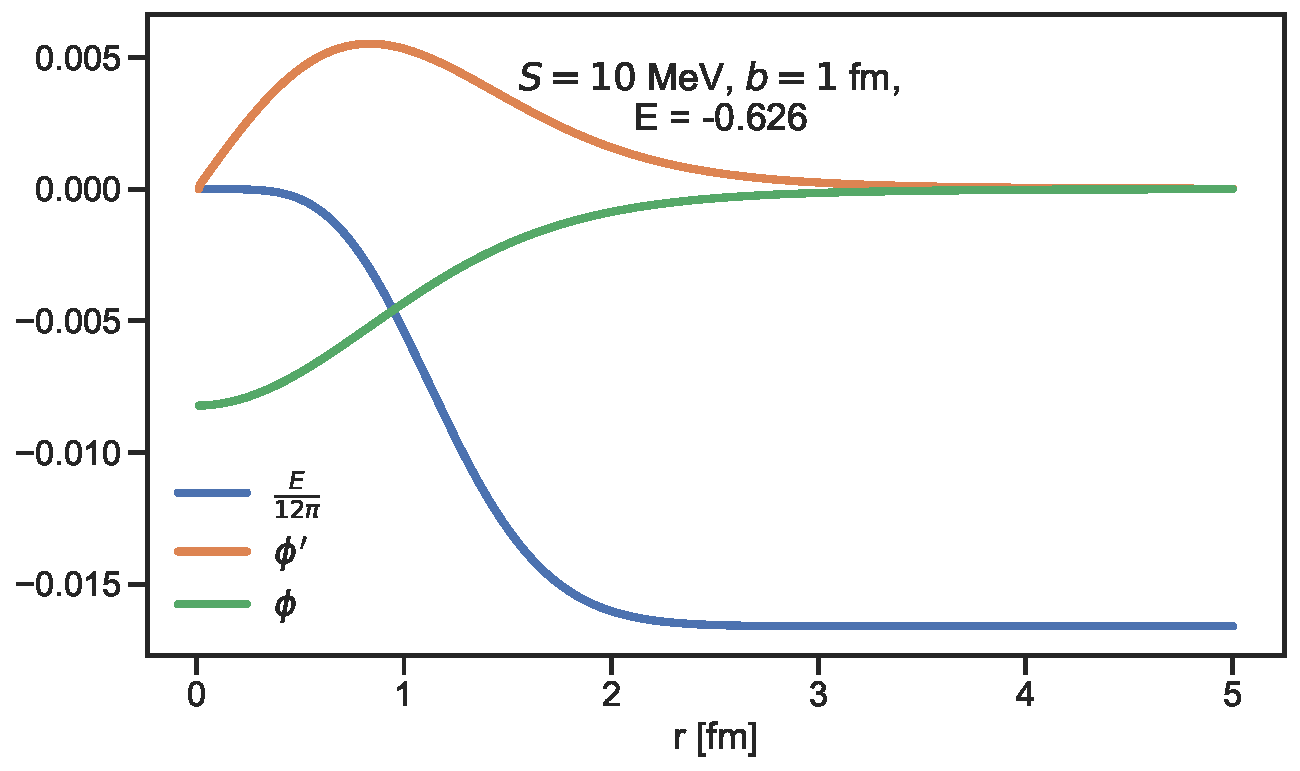
\includegraphics[width=\linewidth]{Figures/Integralplot.pdf}
	\end{sidecaption}
\end{figure}
Also, note that since we expect the energy to be less than zero it makes sense for the wave function to be negative since all other terms in the integral in equation \eqref{system} are positive. It might appear strange to have a negative wave function, $\phi(r)$ but there are two things to note. One can add an arbitrary phase to equation \eqref{2wavefunc} and flip the sign. Also for all calculations, we are only interested in the norm-square of the wave function. The energy for the parameters shown in figure \ref{fig:integralplot} is $E = -0.626 \, \text{MeV}$ and this value is very sensitive to the parameters $S$ and $b$ since they enter in the form factor as seen in equation \eqref{formfactoreq} and as mentioned in section \ref{sec:model} this gives the physical mass of the proton--it's importance will be clear later when comparing the discussion the mass contribution from virtual pion in section \ref{sec:PionPhotoproduction}.

Since we cannot allow the wave function to extend to infinity numerically we must introduce some cut-off. Since the wave function of the pion-nucleon system has a built-in range parameter $b$ it is natural to let the cut-off be proportional to this parameter.
Within the regime of nuclear physics, we expect the wave function to extend up to a length within the order of magnitude of ten Fermi. Quantitatively this means a small constant of proportionality $\mathcal{O}(0.01)$ in front of $r_\text{min}$ and another constant $\mathcal{O}(1)$ in front of $r_{\text{max}}$. Numerically, a constant of proportionality for $r_{\text{max}}$ and the impact can be seen on figure \ref{fig:multiwavefunction} where the radial wave functions stop after $5r_\text{max}$.
\begin{figure}[H]
	\begin{sidecaption}{Radial wave function for different parameters $S$ and $b$ to illustrate the behavoir on the radial function.}[fig:multiwavefunction]
		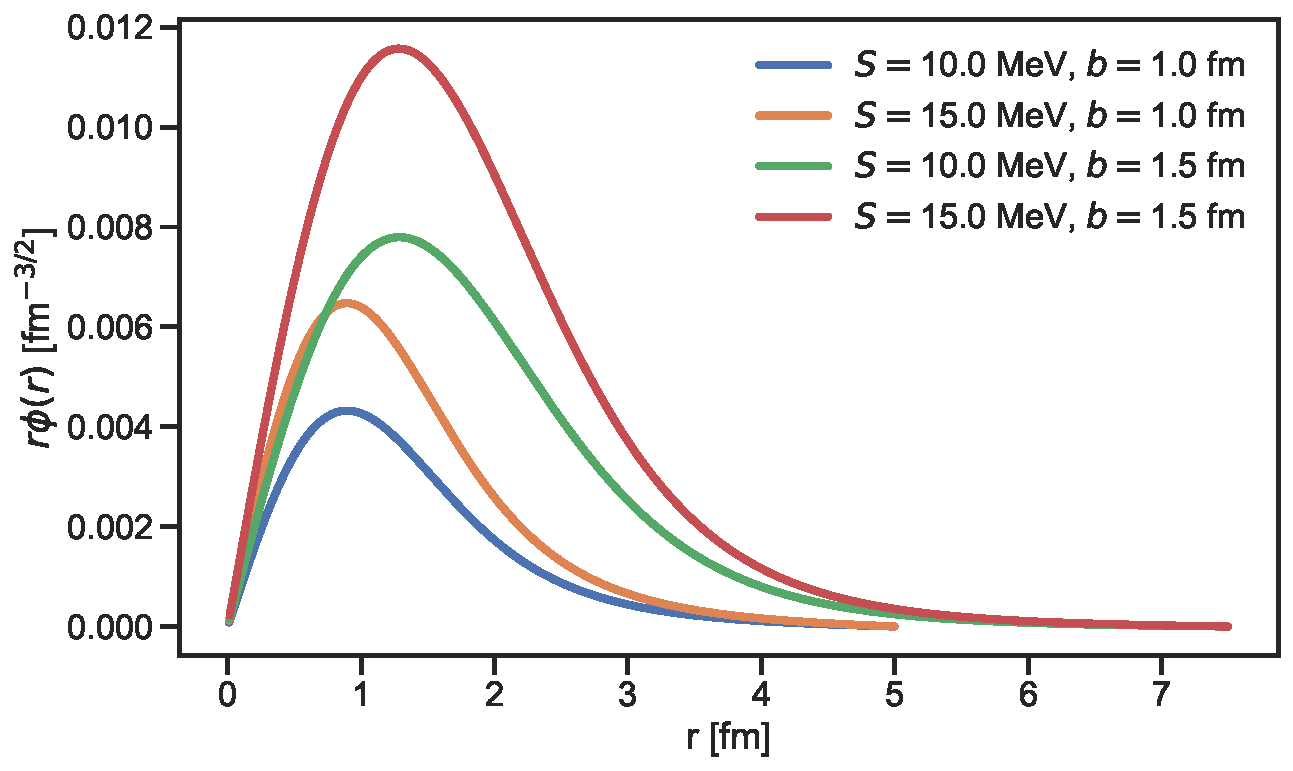
\includegraphics[width=\linewidth]{Figures/multiwavefunction.pdf}
	\end{sidecaption}
\end{figure} 
Figure \ref{fig:multiwavefunction} also illustrates the behaviour of the radial wave functions as the parameters change. As the coupling strength parameter $S$ increases the radial wave function increases. As the range parameter $b$ increases the peak is shifted to this new value. Also, note the unit of the radial wave function. We know the following integral must be dimensionless 
\begin{equation} \label{key}
	\int_V \text{d}^3R \int_V \text{d}^3r \, \abs{ \psi_{N\pi}}^2,
\end{equation}
which means the wave function $\phi(r)$ must have dimensions of fm$^{-5/2}$ and the radial wave function $r\phi(r)$ must have dimensions of fm$^{-3/2}$. Note here the two integrals come from the annihilation of a pion and the normalization of one particle per unit volume respectively.

\subsection{Different form factors}
Compared to conventional interaction models of the nucleus this model has the advantage of having very few parameters. The phenomenological form factor $f(r)$ only consists of an interaction strength $S$ and a range parameter $b$. The form factor can take many different forms yielding different wave function solutions which in turn changed the energy. The formalism in \ref{sec:numericalconsiderations} is very flexible so changes in the form factor and here we explore how different form factors impact the wave function. The form factors must all decrease as a function of $r$ since we constrain the system to short-range forces. The solutions on figure \ref{fig:multiwavefunction} assumes the form factor from equation \ref{formfactoreq} which is Gaussian. A priori we do now know anything about the form factor and it might as well be Yukawa like
\begin{equation}\label{YukawaForm}
	f(r) = \frac{S}{b}\frac{\exp{-\frac{r}{b}}}{r}.
\end{equation}
Figure \ref{integralplotYukawa} shows the radial wave functions if the form factor is Yukawa like
\begin{figure}[H]
	\begin{sidecaption}{}[fig:integralplotYukawa]
		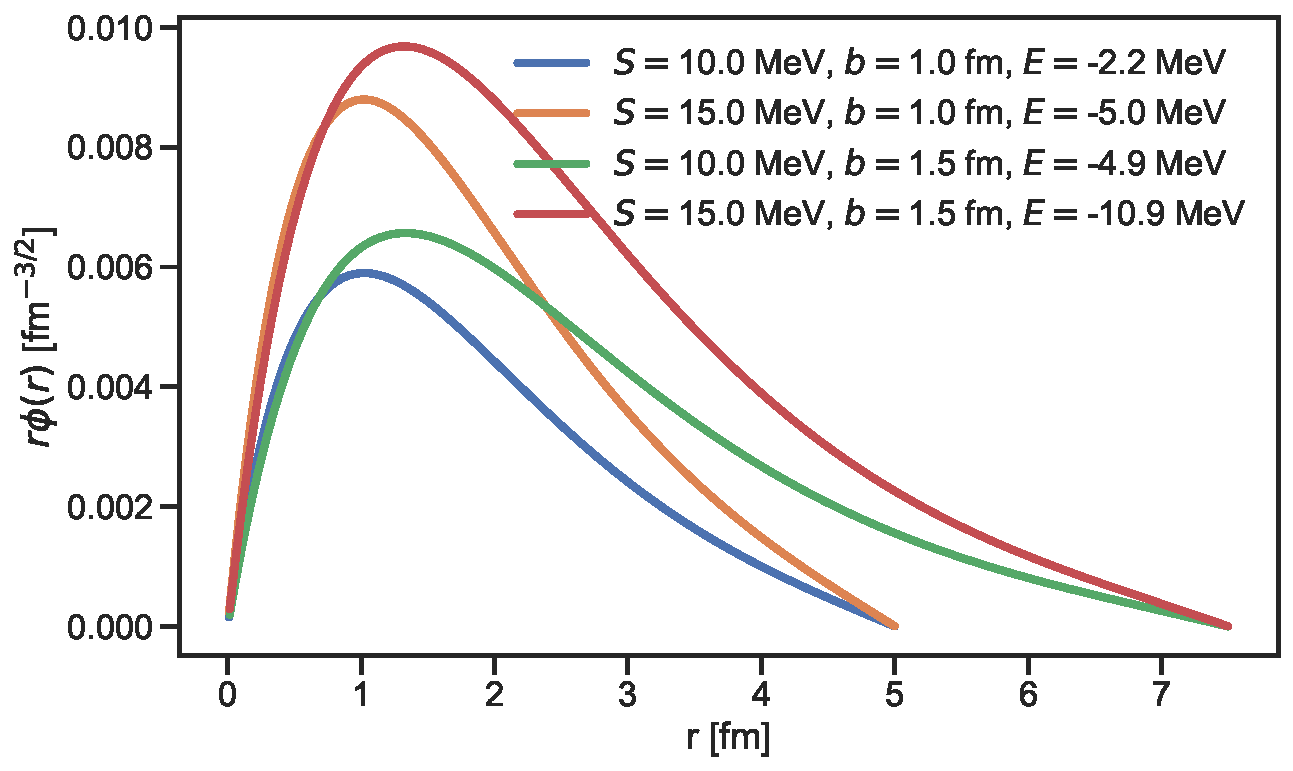
\includegraphics[width=\linewidth]{Figures/multiwavefunctionYukawa.pdf}
	\end{sidecaption}
\end{figure}
The shapes of the radial wave functions are similar to the Gaussian case but the energies do not match due to the $r^2/b^2$ dependency in the Gaussian case. One could argue for a Yukawa-like form factor but with a gaussian exponential and the energies are the same within a few MeV but this defeats the purpose of a Yukawa form. An exponential form factor would make the radial wave function too long to describe the nuclear range since we are constrained to about 15 fm.  
\subsection{Relativistic Expansion}
As described in section \ref{sec:model} we are using the Schrödinger equation which hints at a non-relativistic limit of the pion-nucleon system. We also know the pion is virtual which means under a potential barrier. An avant-garde idea is to do relativistic expansion of the kinetic term which depends on the relative coordinate $\vec{r}$. 


%
The pion is virtual which makes the velocity of the particle hard to estimate--nonetheless we can do an expansion of the kinetic operator and see how this affects the model. To account for relativistic effects we can replace the kinetic term, $K_{\vec{r}}$ in \eqref{SE}
\begin{equation}
	K_{\vec{r}}\rightarrow K_{\vec{r},\text{rel}} = \sqrt{p^2 c^2+\mu_{N\pi}^2 c^4} = \mu_{N\pi} c^2 \bigg(\sqrt{1+\frac{p^2}{\mu_{N\pi}^2 c^2}}-1 \bigg),
\end{equation}
where $\mu_{N\pi}$ is the reduced mass of the nucleon-pion system. This leads to a new system of equations and these solutions can be compared to the non-relativistic limit to deduce which relativistic regime dominates the system. Starting from \eqref{SE2}
\begin{equation}
	f(r) (\vec{\tau} \cdot \vec{\pi})(\vec{\sigma}\cdot \vec{r})\psi_p + \mu_{N\pi} c^2 \bigg(\sqrt{1+\frac{p^2}{\mu_{N\pi}^2 c^2}}-1 \bigg)\psi_{N\pi} = (E-m_{\pi}c^2)\psi_{N\pi},
\end{equation}
This equation turns out to be divergent and we must therefore resort to an approximation. The kinetic energy is expanded
\begin{equation}
	K_{\vec{r},\text{rel}} = \mu_{N\pi} c^2\sqrt{1+\frac{p^2}{\mu_{N\pi}^2}}-\mu_{N\pi} c^2 \approx \frac{p^2}{2\mu_{N\pi}}-\frac{p^4}{8\mu_{N\pi}^3 c^2}
\end{equation}
This means we get an extra term in \eqref{SE22} yielding
\begin{equation}\begin{split}\label{SErel}
		(\vec{\tau\cdot\vec{\pi}})(\vec{\sigma}\cdot\vec{r})f(r)  \frac{p\uparrow}{\sqrt{V}}+\left(\frac{p^2}{2\mu_{N\pi}}-\frac{p^4}{8\mu_{N\pi}^3 c^2} \right)(\vec{\tau}\cdot\vec{\pi})(\vec{\sigma}\cdot\vec{r})\frac{p\uparrow}{\sqrt{V}}\phi(r) \\ \quad= (E-m_\pi c^2) (\vec{\tau\cdot\vec{\pi}})(\vec{\sigma}\cdot\vec{r}) \phi(r)\frac{p\uparrow}{\sqrt{V}},
	\end{split}
\end{equation}
Using the vector operators yields the following expression\footnote{\begin{align*}
		\nabla^4(\vec{r}\phi(r))=\vec{r}\left(\phi^{(4)}+\frac{6}{r}\phi^{(3)}\right)
\end{align*}}
\begin{equation}
	f(r)-\frac{\hbar^2}{2\mu_{N\pi}}\bigg( \phi^{(2)}(r)+\frac{4}{r}\phi^{(1)}(r) \bigg)-\frac{\hbar^4}{8\mu_{N\pi}^3 c^3}\bigg(\phi^{(4)}(r)+\frac{6}{r}\phi^{(3)}(r)\bigg)=(E-m_\pi c^2)\phi(r),
\end{equation}
where the exponent, $(n)$, is the order of the differentiation. This leads to a system of equations given by
\begin{equation} \label{systemrel}
	\left.
	\begin{array}{ll}
		12\pi \int_0^\infty  \text{d}r \, f(r) \phi(r) r^4  = E \\
		f(r)-\frac{\hbar^2}{2\mu_{N\pi}}\big( \phi^{(2)}(r)+\frac{4}{r}\phi^{(1)}(r) \big)-\frac{\hbar^4}{8\mu_{N\pi}^3 c^3}\big(\phi^{(4)}(r)+\frac{6}{r}\phi^{(3)}(r)\big)=(E-m_\pi c^2)\phi(r)
	\end{array}
	\right \} 
\end{equation}
This system is a fourth-order differential equation coupled to an integrodifferential equation and is solved using the boundary value problem technique. The boundary conditions can be found using the same considerations as in the previous section. For $r\rightarrow \infty$ the dominating terms are 
\begin{equation}
	\phi^{(4)}(r) = \frac{-8\mu_{N\pi}c^2}{\hbar^4}(E-m_\pi c^2)\phi(r)-\frac{4\mu^2_{N\pi}c^2}{\hbar^2}\phi(r)^{(2)}
\end{equation}
The solutions are shown in figure \ref{fig:integralplot_relativistic} where only $\phi(r)$ and $\phi(r)^{(1)}$ are included
\begin{figure}[H]
	\begin{sidecaption}{Boundary value problem solutions for the relativistic expansion. The plot is generated using a tolerance of $10^{-3}$. The energy convergence is scaled.}[fig:integralplot_relativistic]
		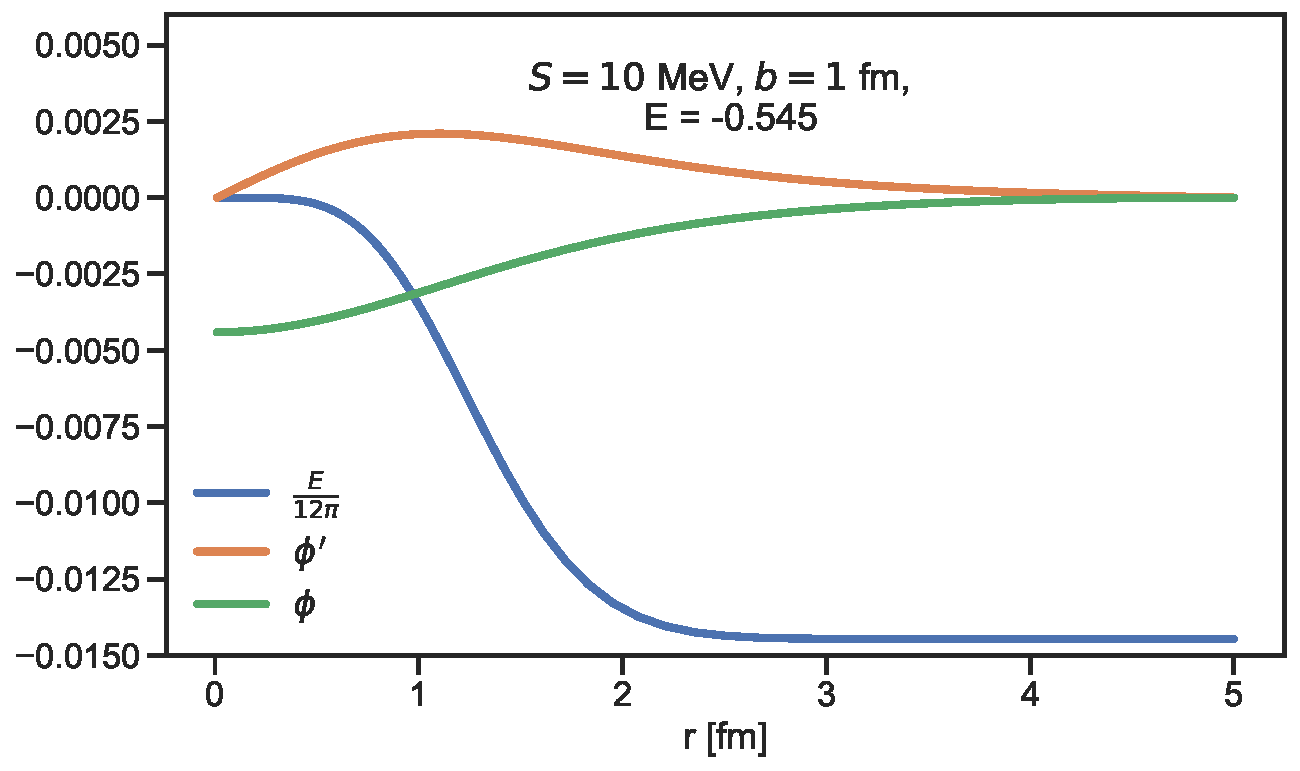
\includegraphics[width=\linewidth]{Figures/Integralplot_relativistic.pdf}
	\end{sidecaption}
\end{figure}
We gain information about the system both from the wave function and the energy and we consider these two components of figure \ref{fig:integralplot_relativistic} separately. The radial wave function of the system can be seen in figure \ref{fig:relativistic_comparison}
\begin{figure}[H]
	\begin{sidecaption}{Relativistic (dashed) and non-relativistic radial wave functions for three different parameters. The matching colours have the same parameters}[fig:relativistic_comparison]
		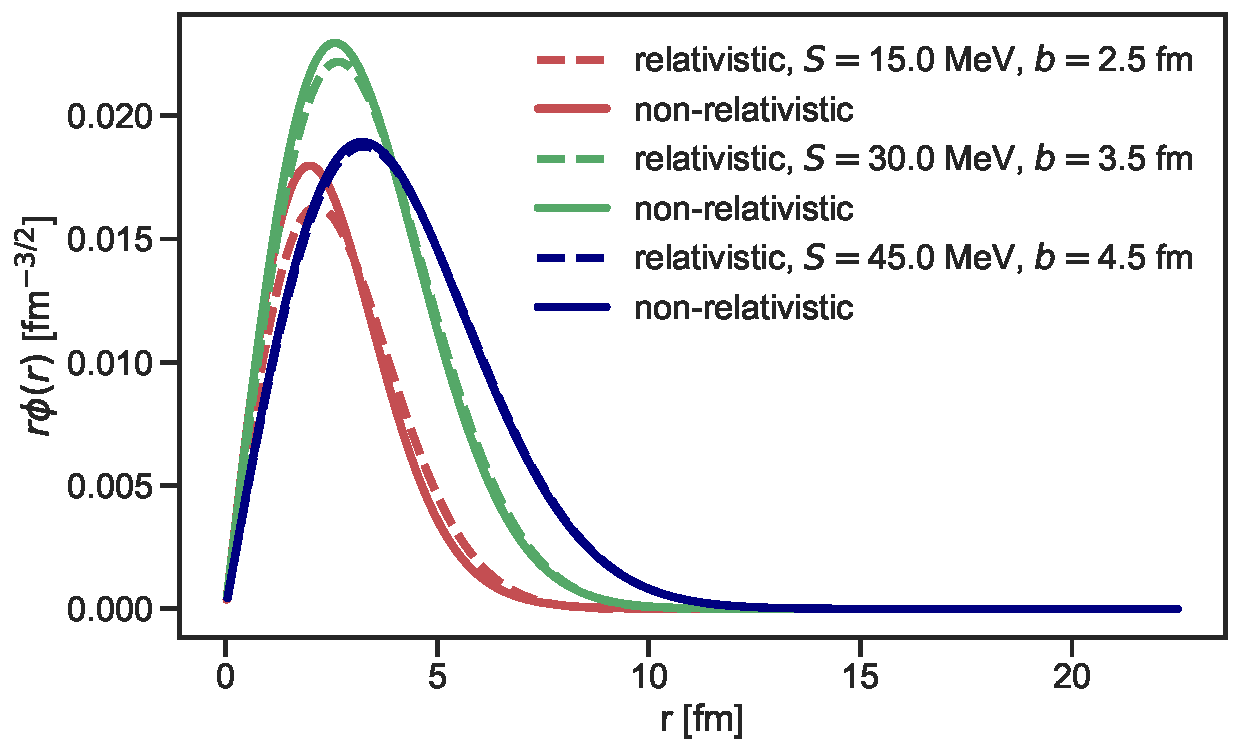
\includegraphics[width=\linewidth]{Figures/rela_vs_nonrela_radial.pdf}
	\end{sidecaption}
\end{figure}
The radial wave functions are similar with the lowest strength parameter $S$ and range parameter $b$ having the largest difference. This can be explained by considering equation \eqref{systemrel}. The form factor $f(r)$ depends explicitly on the ratio between these two parameters in the same way in the relativistic limit as in the non-relativistic limit. However, the form factor can change by orders of magnitude by varying the two parameters and this will only affect the solution $\phi(r)$ regarding when the form factor vanishes and the $r\rightarrow \infty$ limit applies. This also means we should expect the energy ratio between the non-relativistic equation \eqref{system} and equation \eqref{systemrel} to approach 1 as the range parameter $b$ increases since this decreases the impact of the form factor. This is shown in figure \ref{fig:b_convergence} where the energy ratio is given by
\begin{equation} \label{energyratio}
	E_R = \frac{E_\text{relativistic}}{E_\text{non-relativistic}}.
\end{equation}
\begin{figure}[H]
	\begin{sidecaption}{The energy ratio $E_\text{rel}/E_\text{nonrel}$ shown as a function of the range parameter $b$ for a Gaussian form factor given by equation \eqref{formfactoreq}}[fig:b_convergence]
		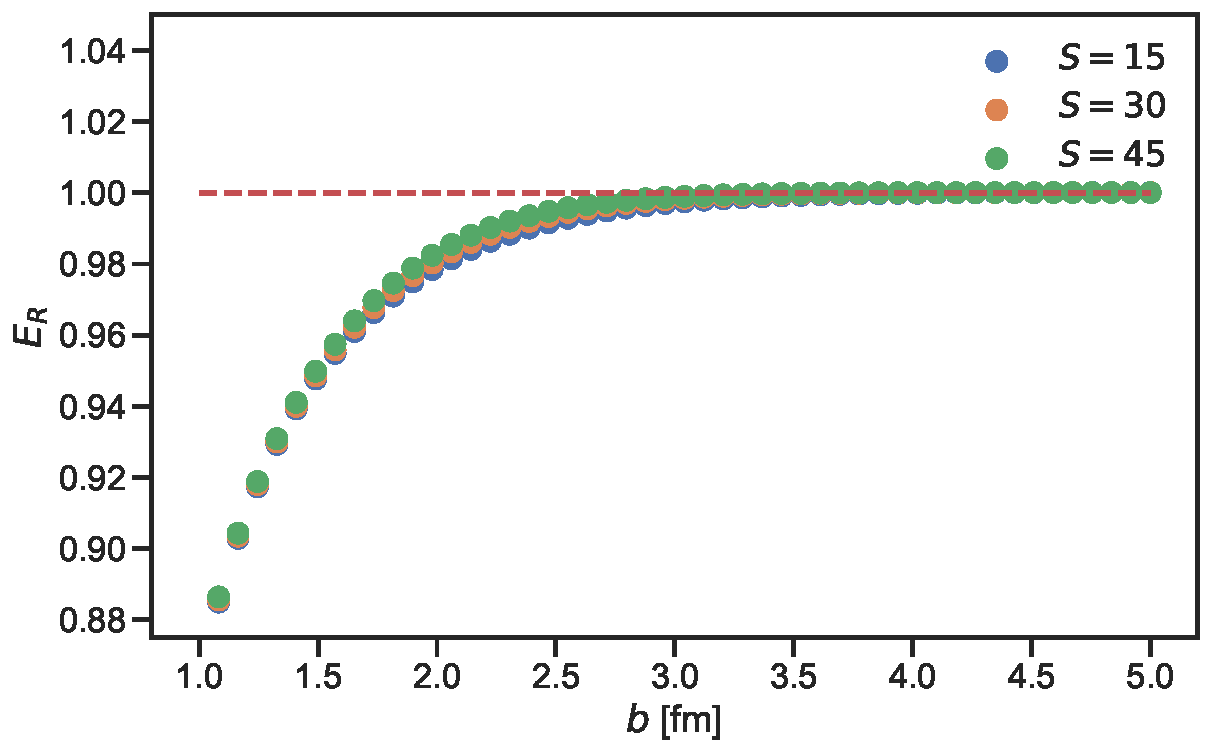
\includegraphics[width=\linewidth]{Figures/bconvergence.pdf}
	\end{sidecaption}
\end{figure}
We can apply the same logic to the system of equations with a Yukawa-like form factor as in equation \eqref{YukawaForm} and we expect the same convergence. This is shown on figure \ref{fig:b_convergenceYukawa}
\begin{figure}[H]
	\begin{sidecaption}{The energy ratio $E_\text{rel}/E_\text{nonrel}$ shown as a function of the range parameter $b$ for a Yukawa-like form factor given by equation \eqref{YukawaForm}}[fig:b_convergenceYukawa]
		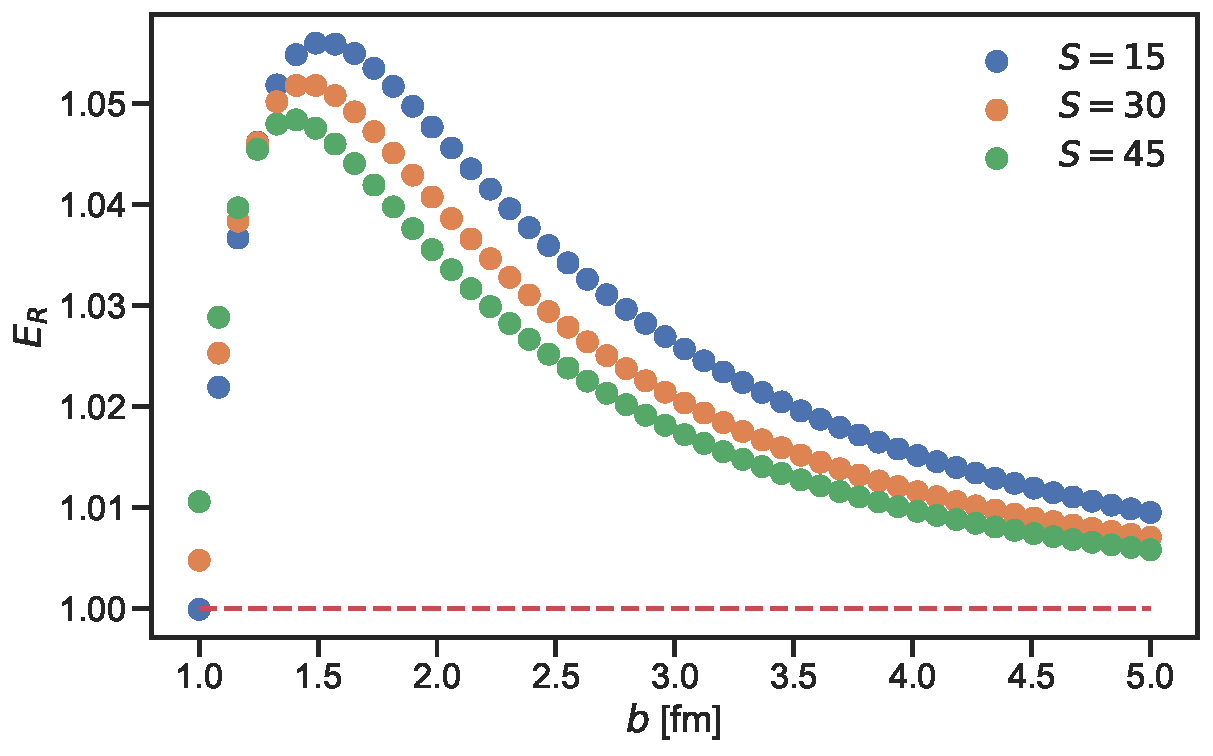
\includegraphics[width=\linewidth]{Figures/bconvergenceYukawa.pdf}
	\end{sidecaption}
\end{figure}
The pion is virtual and hence in a classically forbidden region but we can still estimate which relativistic regime dominates the system. Both in terms of the radial wave function and in terms of the energy ratio relativistic effects are negligible. This result holds for different form factors since they most all decrease a function of $r$. 

\subsection{Nuclear Effective Field Theory operator}
The construction of the most general chiral Lagrangian is based on the theory of the non-linear realization of symmetry. The baryon-number-conserving chiral Lagrangian can be split into pieces with even numbers of fermion fields where in this section we will focus on 
\begin{equation}
	\mathcal{L} = N^\dagger \left(i\mathcal{D}_0+\frac{\vec{\mathcal{D}}^2}{2m_N} \right)N+\frac{g_A}{2f_\pi}N^\dagger\vec{\tau}N\cdot \vec{D}\vec{\pi},
\end{equation}
where the second term is very similar to the creation operator $W$ from equation \eqref{W}--only the $\vec{r}$ is replaced by $\nabla_{\vec{r}}$. The general operator is constructed in such a way that parity, isospin and spin are conserved and there is some freedom in the choice of the distance operator. In this section, we explore the differences, if any, by constructing the nuclear model with explicit mesons with the operator as is it defined in chiral effective field theory. We assume the following form of the wave function of the proton and the system consisting of a nucleon and a single pion
\begin{equation}
	\psi_p = p\uparrow\frac{1}{\sqrt{V}}, \quad \psi_{N\pi} = (\vec{\tau}\cdot \vec{\pi})(\vec{\sigma}\cdot \frac{\partial}{\partial\vec{r}})p\uparrow \frac{1}{\sqrt{V}}\phi,
\end{equation}
where $\vec{\tau}$ and $\vec{\sigma}$ are vectors consisting of Pauli matrices acting on isospin and spin space on the nucleon respectively. $\vec{\pi}$ is the isovector of pions. We now construct an operator to create and annihilate a pion
\begin{align}
	W & = (\vec{\tau}\cdot \vec{\pi})(\vec{\sigma}\cdot \frac{\partial}{\partial\vec{r}})f(r) \\
	W^\dagger & = \int_V \text{d}^3 r \, (\vec{\tau}\cdot \vec{\pi})^\dagger(\vec{\sigma}\cdot \frac{\partial}{\partial\vec{r}})^\dagger f(r),
\end{align}
where $f(r)$ is a form factor. The annihilation operator must contain the integral to remove the coordinate of the pion. This leads to the following Schrödinger equation
\begin{equation}
	\mqty[K_{\vec{R}} & W^\dagger \\ W & K_{\vec{R}}+K_{\vec{r}}+m_\pi c^2]\mqty[\psi_p \\ \psi_{N\pi}]=E\mqty[\psi_p \\ \psi_{N\pi}],
\end{equation}
which is expanded
\begin{align}\label{CEFTint}
	12\pi \int_0^\infty \text{d}r \, \frac{\partial^2}{\partial r^2}r^2f(r)\phi(r) =E \\
	\frac{\partial}{\partial r}f(r)-\frac{2\hbar^2}{\mu_{N\pi}} \frac{\partial^3}{\partial r^3}\phi(r) = (E-m_\pi c^2)\frac{\partial}{\partial r}\phi(r)\label{CEFT2}.
\end{align}
Assume the form factor is on the following form
\begin{equation}
	f(r) = \frac{S}{b}\text{e}^{-r^2/b^2}
\end{equation}
which yields
\begin{equation}
	\frac{\partial}{\partial r} f(r) = \frac{-2r}{b^2}f(r), \quad \frac{\partial^2}{\partial r^2}=-\frac{2(b^2-2r^22)}{b^4}f(r).
\end{equation}
The terms inside the integral in equation \eqref{CEFTint} 
\begin{align}
	\frac{\partial^2}{\partial r^2}(r^2f(r)\phi(r)) & = 2rf(r)\phi(r)+2rf^\prime(r)\phi(r)+r^2f(r)\phi ^\prime(r)
	\\&+2rf^\prime(r)\phi(r)+r^2f^{\prime\prime(r)}\phi(r)+r^2f^\prime(r)\phi^\prime(r)\\
	&+2rf(r)\phi(r)+r^2f^\prime(r)\phi^\prime (r)+r^2f(r)\phi^{\prime\prime}(r) \\&\equiv Y(r)
\end{align}
Considering the limits of \eqref{CEFT2} which for large $r$ is
\begin{equation}
	\phi^{\prime\prime\prime}(r) =\frac{-\mu_{N\pi}}{2\hbar^2}(E-m_\pi c^2)\phi^\prime(r)
\end{equation}
The solution is shown on \ref{fig:EFTplot}
\begin{figure}[H]
	\begin{sidecaption}{The radial wave function using the operator form from an effective field theory.}[fig:EFTplot]
		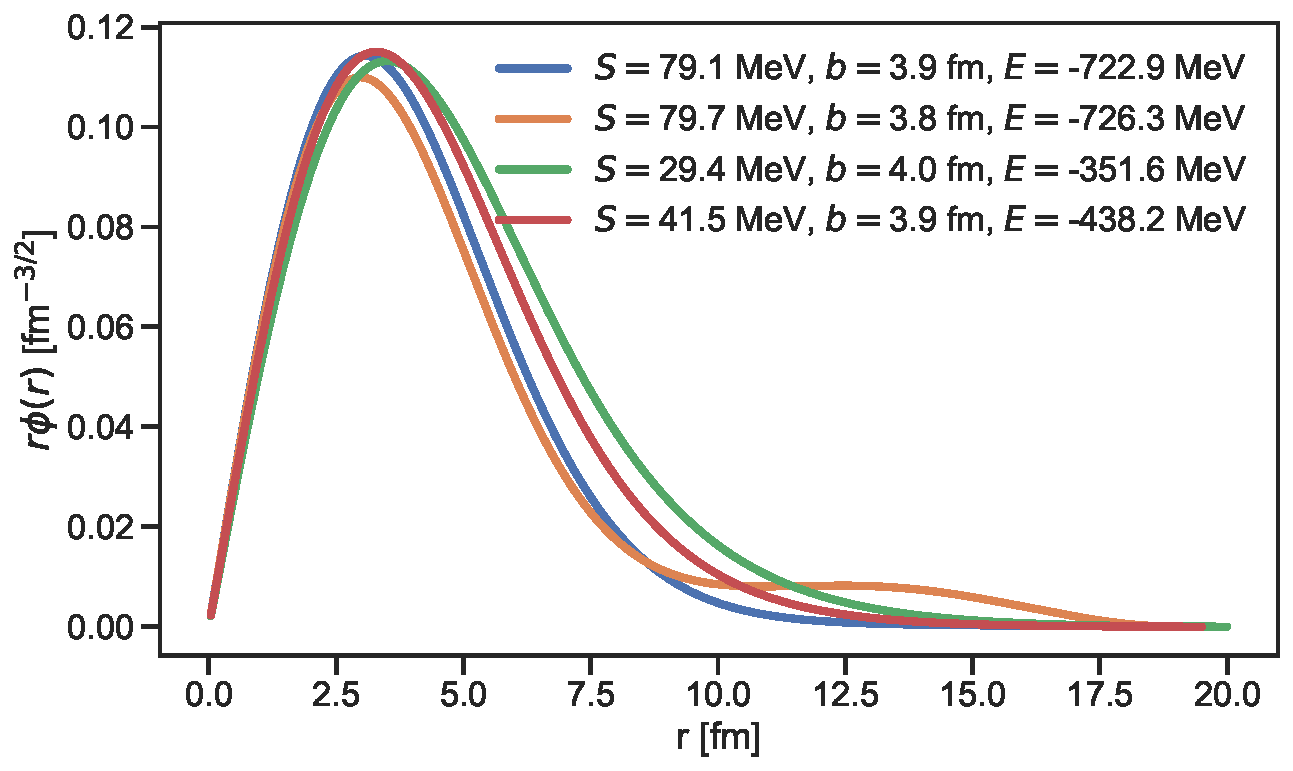
\includegraphics[width=\linewidth]{Figures/EFTradial.pdf}
	\end{sidecaption}
\end{figure}

